
\chapter{Introduction}

In this paper, I am proud to finally introduce the world to \emph{Skedge}, a website I have been developing in various degrees since December 9th, 2013. Skedge began as a weekend side-project for me after spending too much time frustrated with existing tools while trying to find myself a second major to pursue. It wasn't until I briefly presented it at an on-campus RocHack meeting when I realized it had potential to help other students as well, but since, it has always existed in the shadows and in continual ``beta''---unofficial, unsupported and dodging recognition. Until two summers ago, I had never expected it to end up being the subject of my honors senior thesis, so this opportunity represents a rather special privilege for me and, selfishly, an outlet for recognition.

\section{Overview of CDCS}

``Course Description / Course Schedule,'' (or \emph{CDCS} for short) is the University's official tool for browsing through the University's current course catalog. 

\label{fig:cdcs-index}

\subsection{``Better CDCS''}

%%%

\section{Overview of Skedge}

Skedge is a website on which I started rapid development on , and have been developing it on and off since.

Bookmarks

Students, parents, department coordinators, and faculty can all benefit from such tool improvements.

user accounts are lightweight, no login, cookie (browser) based

\ref{fig:sk-index}


\begin{figure}[ht]
    \centering
        \begin{subfigure}[h]{14cm}
            \centering
            \fbox{
                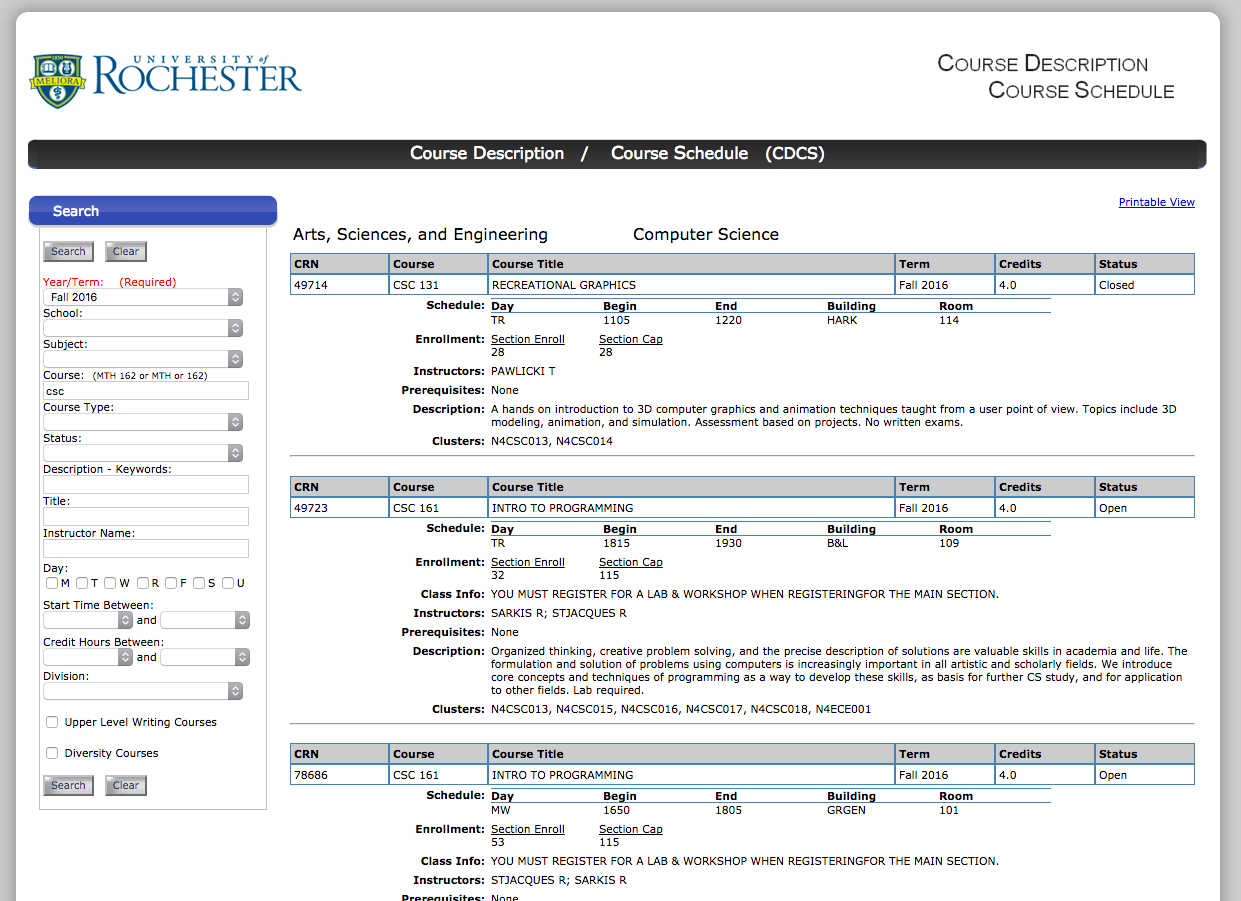
\includegraphics[width=1.00\textwidth]{images/cdcs/index}
            }
            \caption{CDCS, with the search query {\tt csc}}
            \label{fig:cdcs-index}
        \end{subfigure}\\
        \vspace{10pt}\\
        \begin{subfigure}[h]{14cm}
            \centering
            \fbox{
                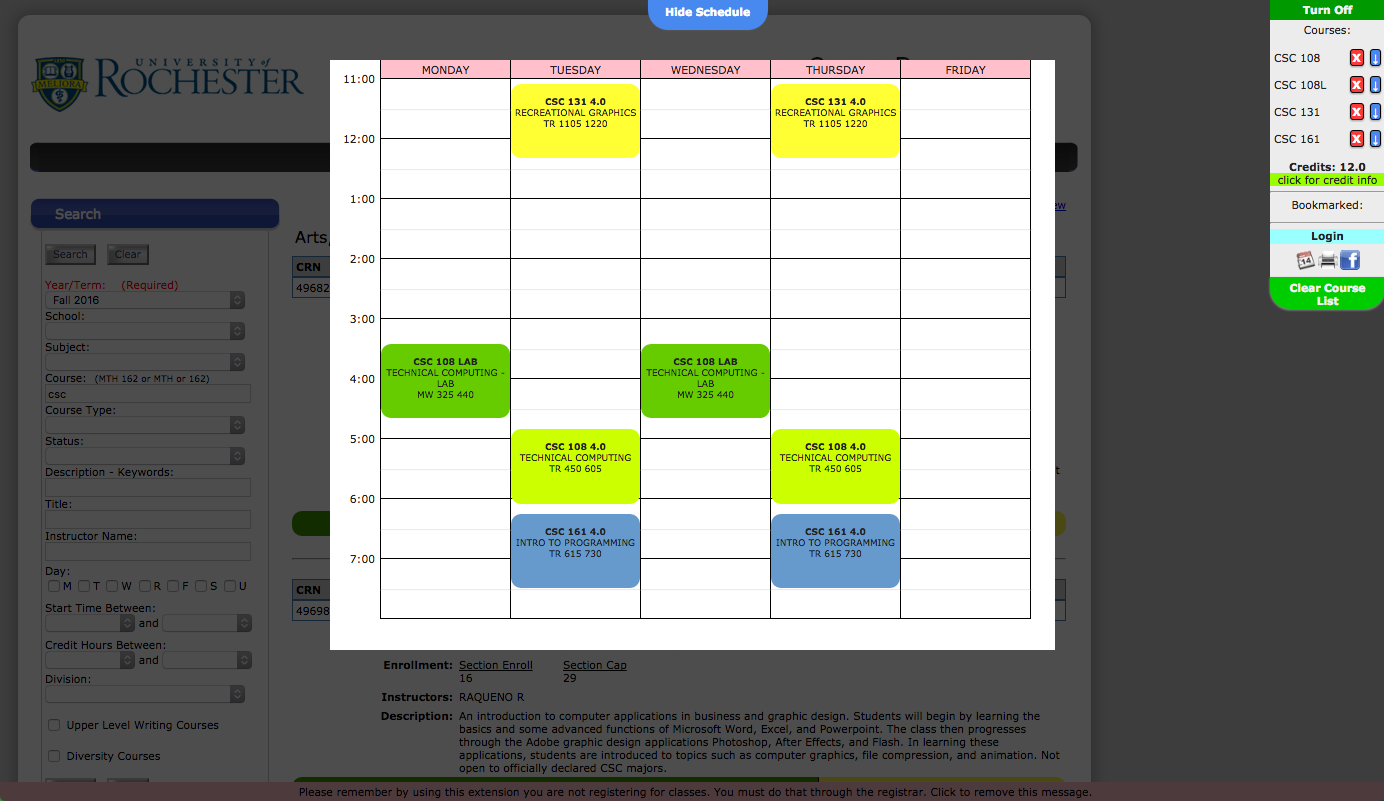
\includegraphics[width=1.00\textwidth]{images/cdcs/better}
            }
            \caption{Better CDCS, a separate browser extension that embeds buttons into the CDCS course results interface, allowing users to add courses to a locally-stored schedule}
            \label{fig:cdcs-better}
        \end{subfigure}
    \caption{CDCS and Better CDCS in their current states}
\end{figure}

\begin{figure}[ht]
    \centering
    \fbox{
        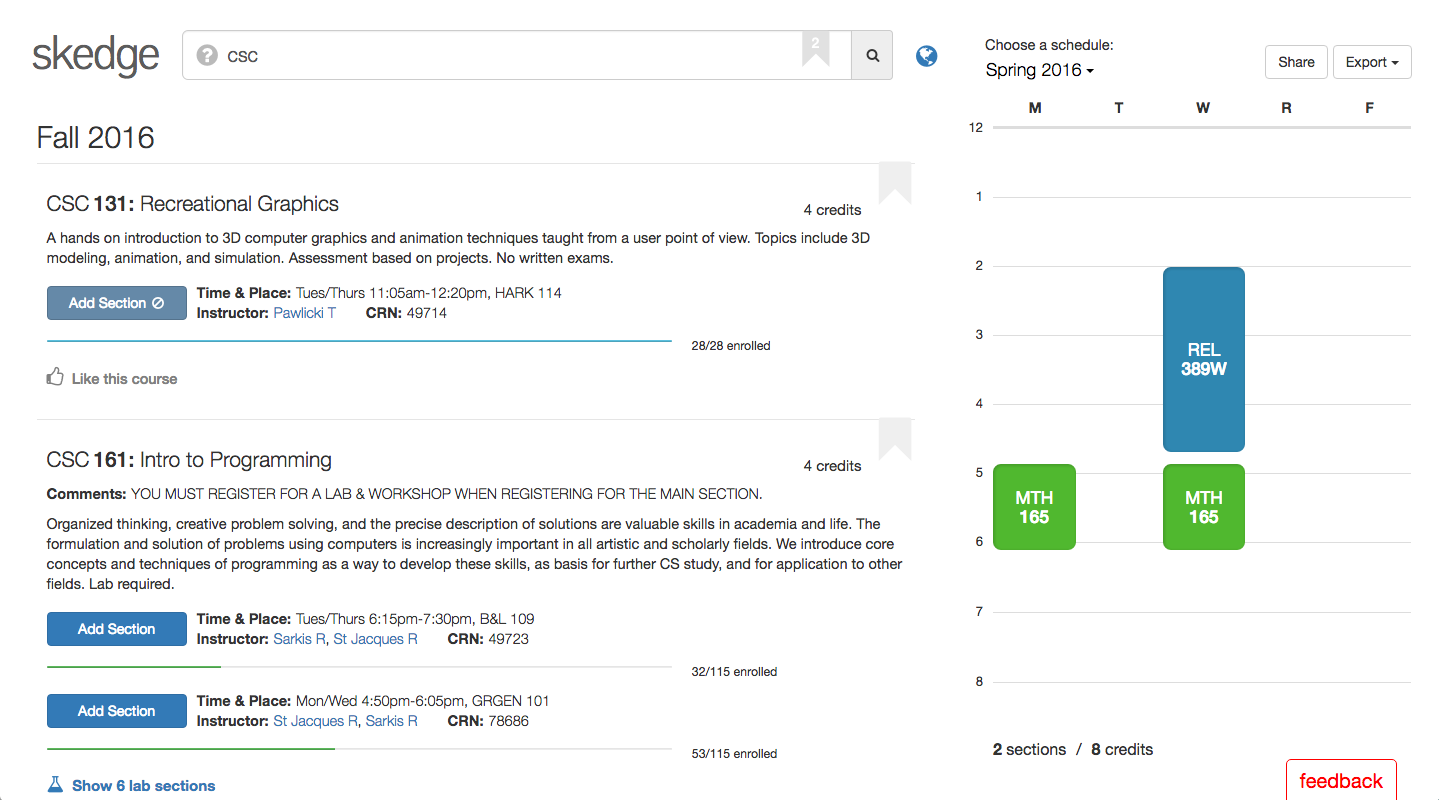
\includegraphics[width=1.00\textwidth]{images/skedge/index}
    }
    \caption[Skedge with the search query {\tt csc}]{Skedge with the search query {\tt csc} and the user's current schedule on the right}
    \label{fig:sk-index}
\end{figure}